\documentclass{beamer}
%
% Choose how your presentation looks.
%
% For more themes, color themes and font themes, see:
% http://deic.uab.es/~iblanes/beamer_gallery/index_by_theme.html
%

% Theme License: https://creativecommons.org/licenses/by/4.0/

\mode<presentation>
{
  \usetheme{default}      % or try Darmstadt, Madrid, Warsaw, ...
  \usecolortheme{default} % or try albatross, beaver, crane, ...
  \usefonttheme{default}  % or try serif, structurebold, ...
  \setbeamertemplate{navigation symbols}{}
  \setbeamertemplate{caption}[numbered]
} 

\usepackage[english]{babel}
\usepackage[utf8x]{inputenc}

\title[Ghidra]{An Introduction to Reverse Engineering}
\author{Jake Vossen}
\institute{Colorado School of Mines - oresec}
\date{2019-03-19}

\begin{document}

\begin{frame}
  \titlepage
\end{frame}

% Uncomment these lines for an automatically generated outline.
%\begin{frame}{Outline}
%  \tableofcontents
%\end{frame}

\section{Introduction}

\begin{frame}{What is Software Reverse Engineering?}

\begin{itemize}
  \item IEEE defines it as ``he process of analyzing a subject system to identify the system's components and their interrelationships and to create representations of the system in another form or at a higher level of abstraction''
  \item Generally is taking a piece of compiled software and analyzing
    it, revealing information about the source code
  \item Often used in security research, but also have implication in
    game emulation and other areas of proprietary software.
\end{itemize}

\vskip 1cm

\end{frame}

\begin{frame}{Why Ghidra?}
  \begin{figure}
    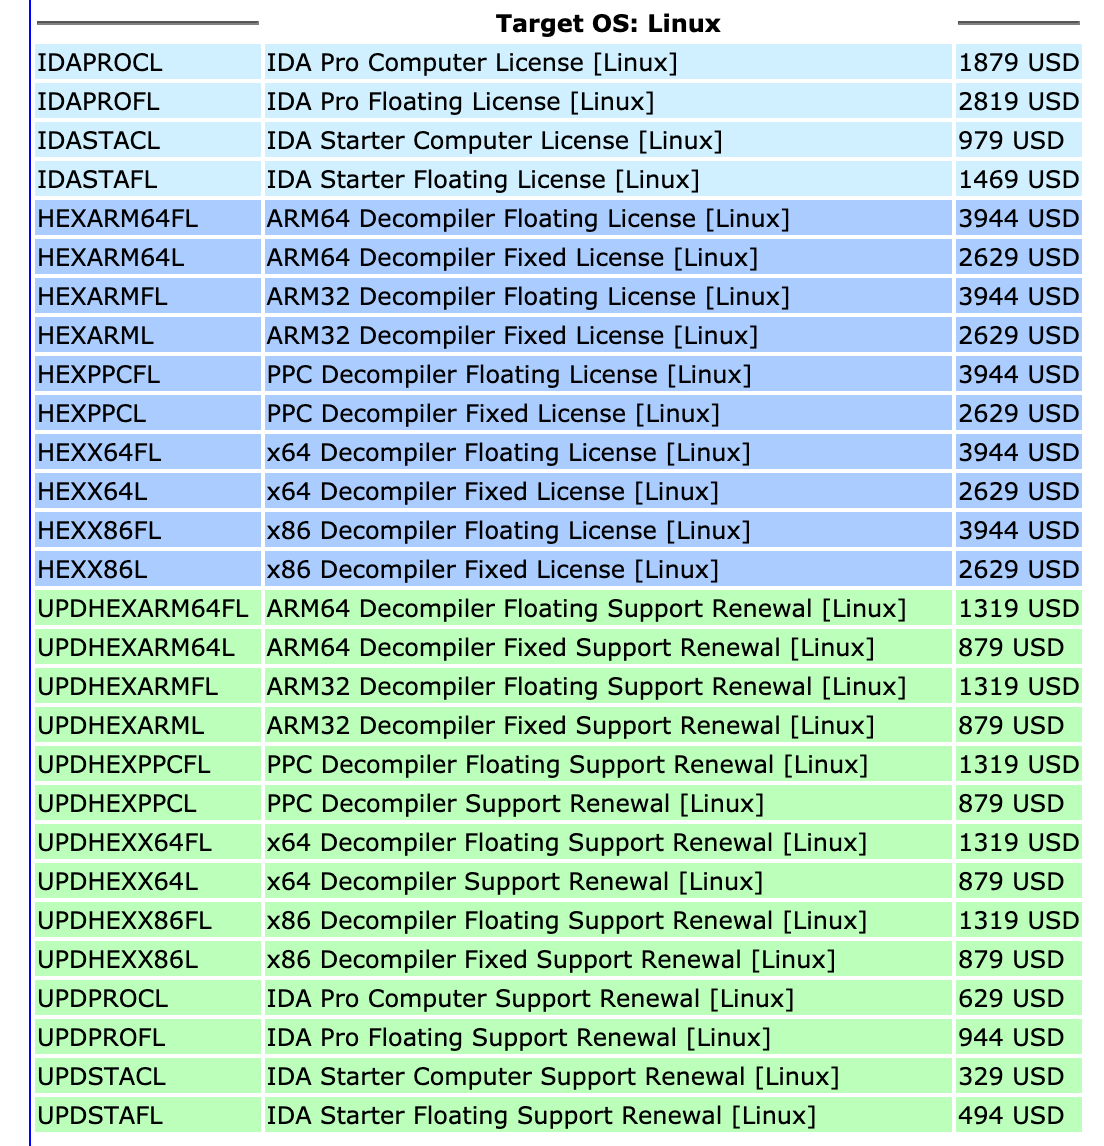
\includegraphics[width=\textwidth]{hex-rays-pricing.png}
    %% \caption{\label{fig:your-figure}Hex Rays Pricing}
  \end{figure}
\end{frame}

\begin{frame}{And if that wasn't enough...}
  \begin{figure}
    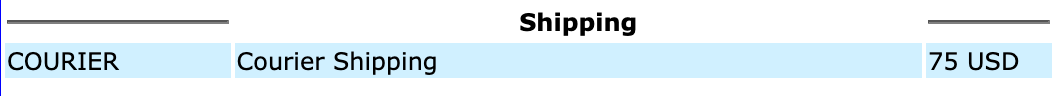
\includegraphics[width=\textwidth]{ida-shipping.png}
    %% \caption{\label{fig:your-figure}Hex Rays Pricing}
  \end{figure}
\end{frame}

% Commands to include a figure:
%\begin{figure}
%\includegraphics[width=\textwidth]{your-figure's-file-name}
%\caption{\label{fig:your-figure}Caption goes here.}
%\end{figure}


\subsection{Mathematics}

\begin{frame}{Readable Mathematics}

Let $X_1, X_2, \ldots, X_n$ be a sequence of independent and identically distributed random variables with $\text{E}[X_i] = \mu$ and $\text{Var}[X_i] = \sigma^2 < \infty$, and let
$$S_n = \frac{X_1 + X_2 + \cdots + X_n}{n}
      = \frac{1}{n}\sum_{i}^{n} X_i$$
denote their mean. Then as $n$ approaches infinity, the random variables $\sqrt{n}(S_n - \mu)$ converge in distribution to a normal $\mathcal{N}(0, \sigma^2)$.

\end{frame}

\end{document}
